\section{Requirements and Inspiration}

The BeachBot project itself was inspired by the images of sand artists like Peter Donnelly and Andres Amador, who manually create large scale sand art at beaches using a rake. Some of the imagery that was found online can be seen in \autoref{fig:sandart_inspiration}.

\begin{figure}
\centering
\begin{subfigure}[c]{1\textwidth}
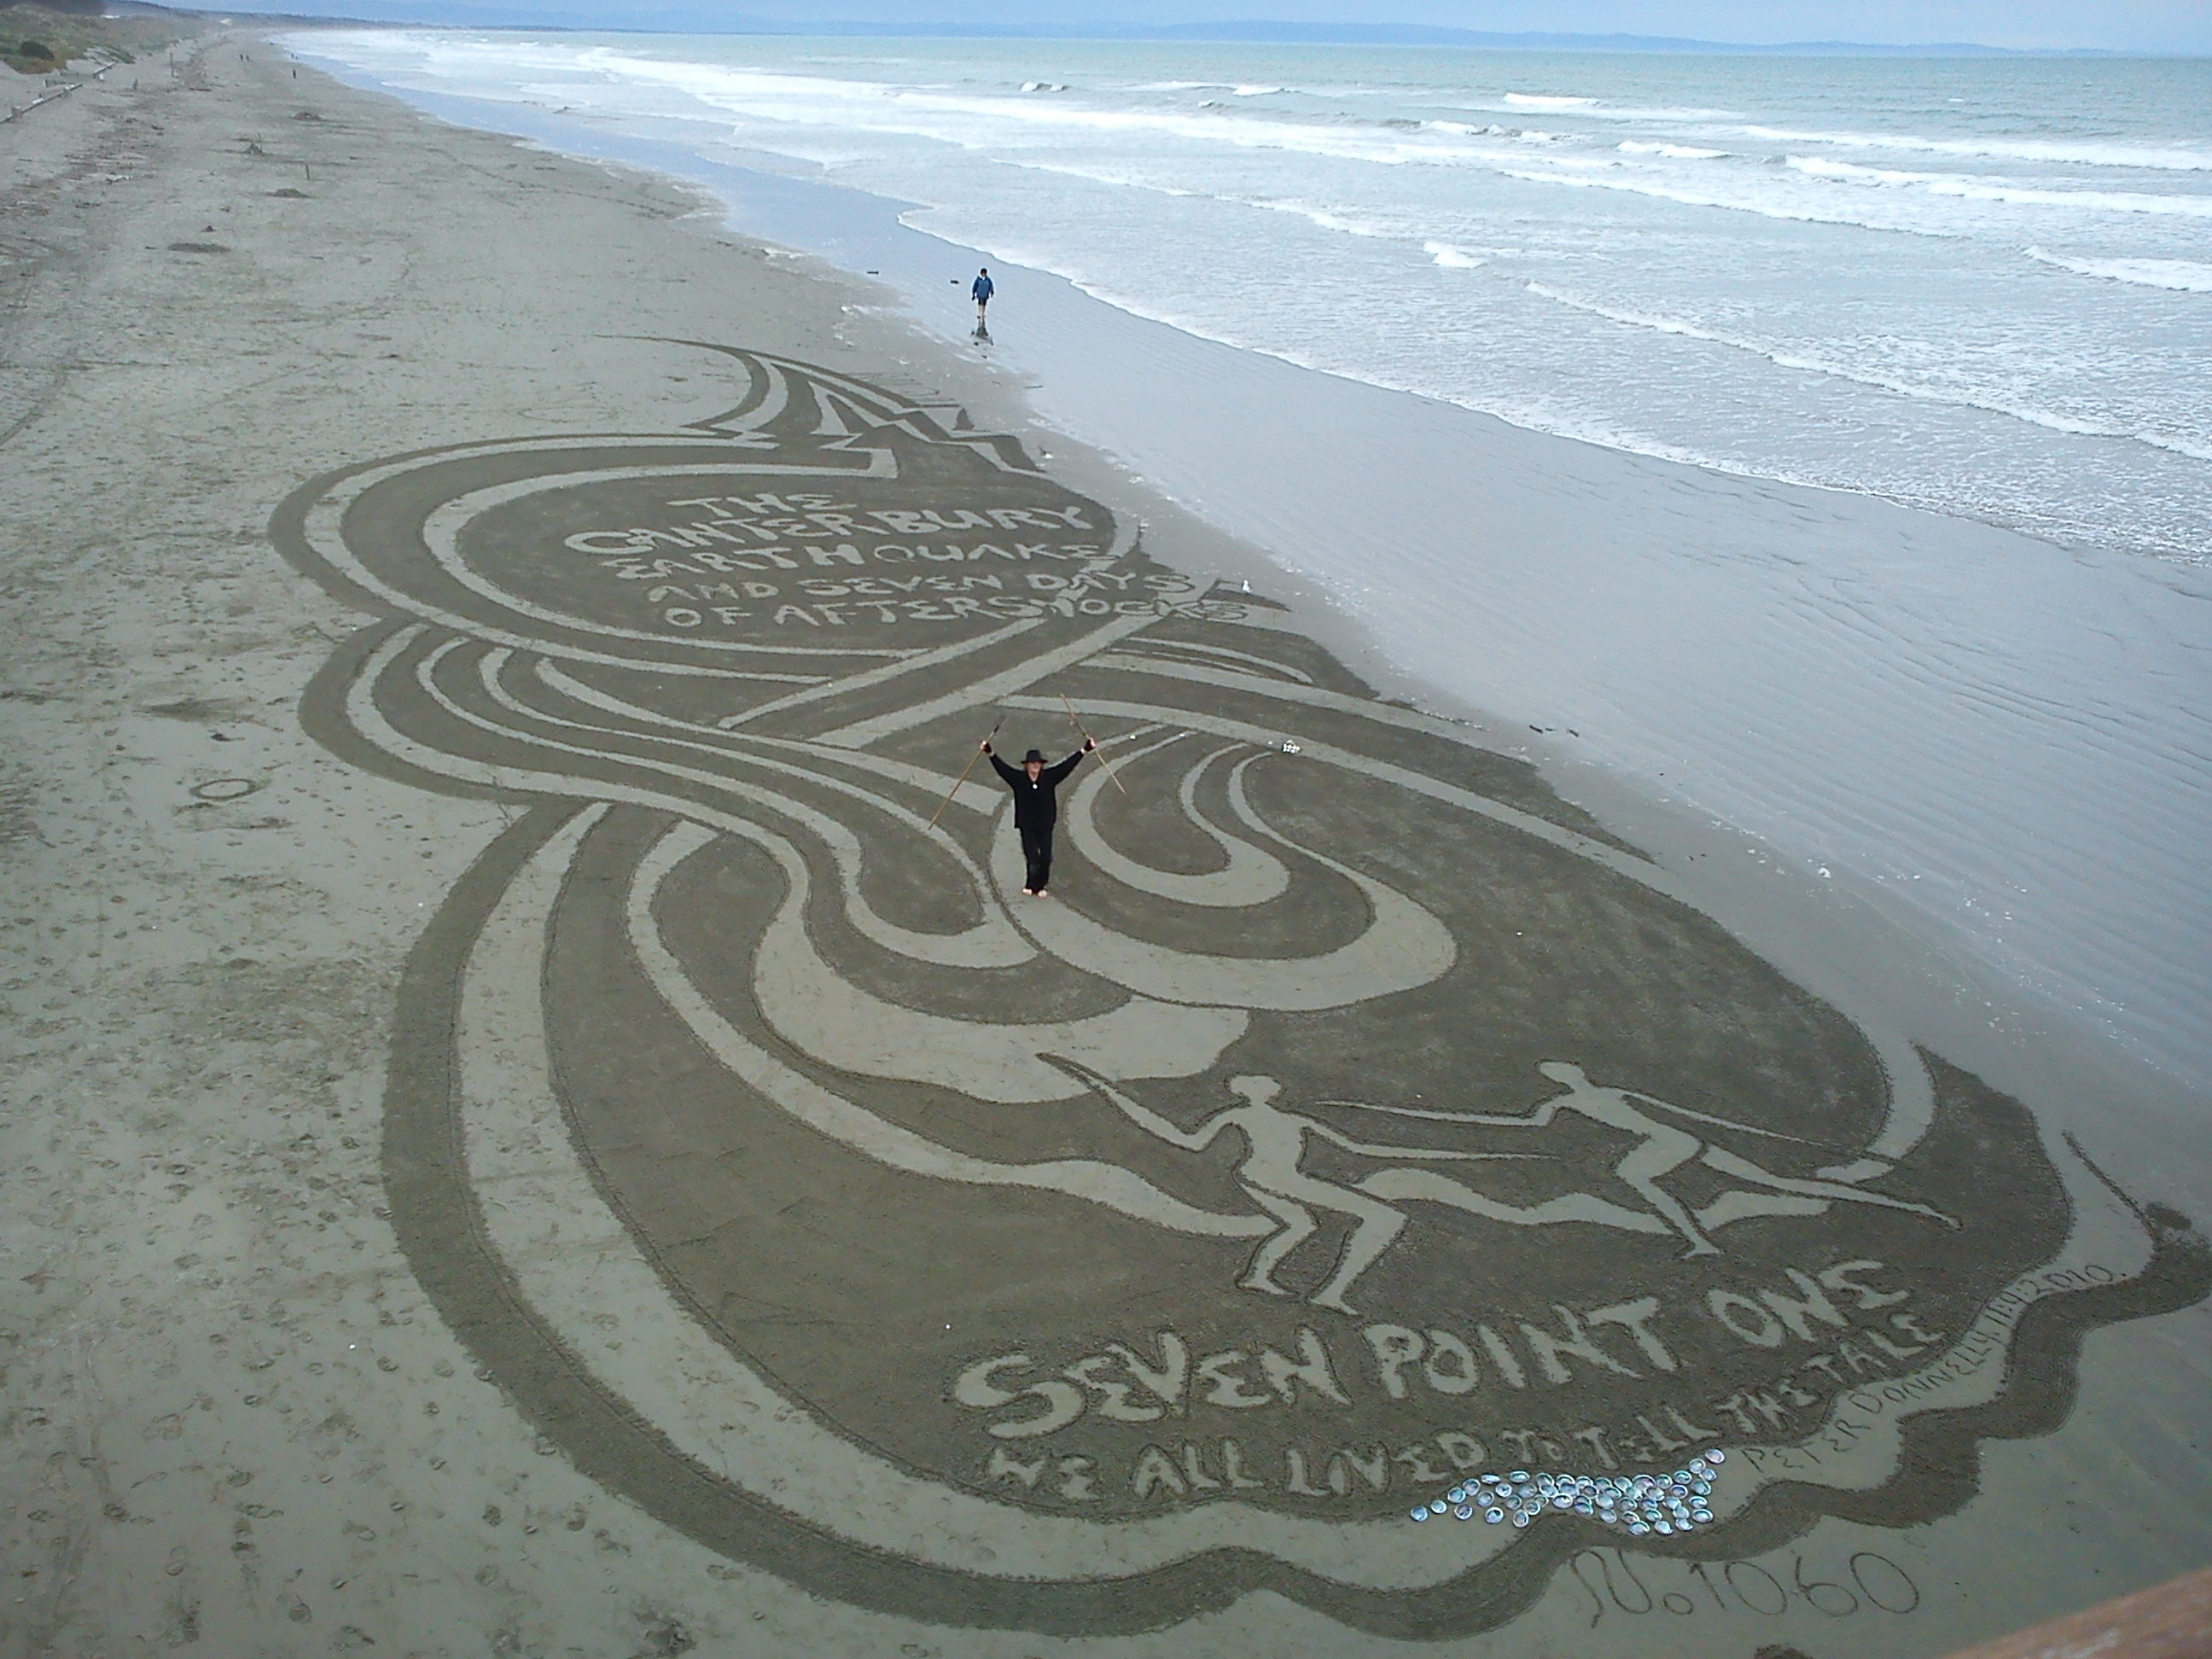
\includegraphics[width=\textwidth]{images/requirements_inspiration/donnelly_1.jpg} 
\caption{Sand drawing by Peter Donnelly. Source: \url{http://becky-garrett.blogspot.ch/2009/03/sand-dancer-peter-donnelly.html}}
\end{subfigure}
\\
\begin{subfigure}[b]{0.46\textwidth}
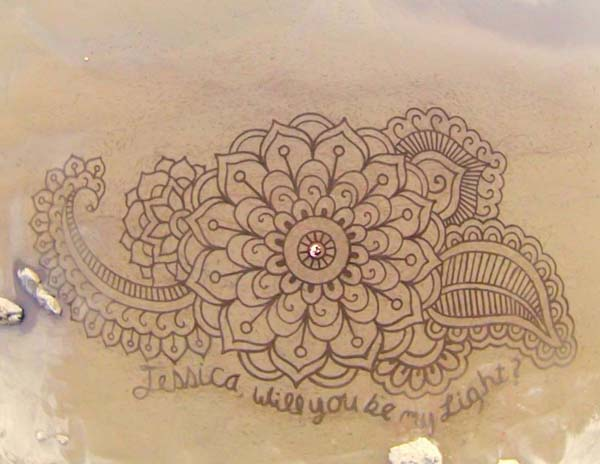
\includegraphics[width=\textwidth]{images/requirements_inspiration/andres_armador_1.jpg} 
\caption{Sand drawing by Andres Amador. Source: \url{http://sftimes.co/?id=25}}
\end{subfigure}
~
\begin{subfigure}[b]{0.46\textwidth}
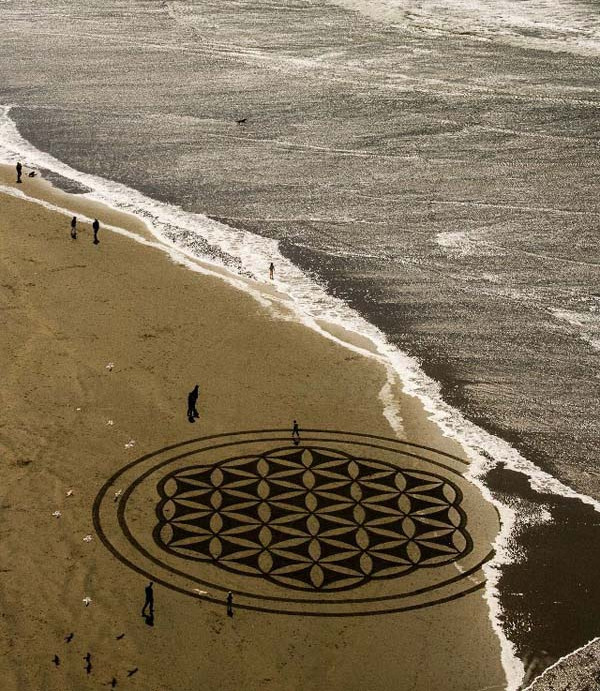
\includegraphics[width=\textwidth]{images/requirements_inspiration/andres_armador_2.jpg} 
\caption{Sand drawing by Andres Amador. Source: \url{http://sftimes.co/?id=25}}
\end{subfigure}
\caption{Various beach drawings by artists}
\label{fig:sandart_inspiration}
\end{figure}

Since the goal of the project is to create drawings similar to those of the artists, the requirements were derived from these sample images.

First of all, the BeachBot should be able to draw lines. But more important is the support of filled areas. While it is relatively straightforward how to drive over lines or curves to draw them, there is no easy solution to derive the path for the filled areas. Not only should the area be covered to the highest extent, but the drawing process should also look interesting and artistic to spectators as well.

Derived from \autoref{fig:sandart_inspiration} is also the requirement that the BeachBot only needs to be able to draw in two colors. Gradients or differently colored areas are unnecessary.

Crossing lines or filled areas should be avoided as good as possible since the balloon wheels and the front wheel leave visible marks on the raked sand (a humanoid has a huge advantage here, since it can jump over the drawn areas). The effect of driving over the drawing depends on the scale. If the drawing is very big, it does not matter much if part of the image is crossed out. 

The input of the path generator should not only be computer readable, but also human editable. Typing in endless lists of coordinates would be tedious in the long run, and having a difficult format to work with would make it hard to collaborate with artists, for example. 
%Therefore the requirement to be able to use a modern graphics editor tool to work with was set. To conform to this requirement we soon decided to use \textit{Inkscape}\footnote{\url{http://inkscape.org}}, a popular open source vector graphics editor, as our input creation tool of choice. Further discussion about vector graphics as input and the steps to integrate a standardized vector graphics format into the path generator are explained in \autoref{sec:why_vector} and \autoref{sec:implementation_svg} respectively.

During the testing phase it was found out, that some of the generated paths needed some manual adjusting. To be able to easily edit the output of the generator program a graphical user interface should be created to work with the output of the generator program. 

In the following sections it will be shown how these requirements were fulfilled and to which extent.

\subsection{The Path Converter}\label{sec:pathconv}

Another bachelor thesis that was written as part of the BeachBot project deals with the rake offset of the robot. The rake is not at the same spot as the turning point of the robot, which leads to errors when the image is drawn in the sand. Therefore, the path converter uses an optimization technique to adjust the path generated by this bachelor thesis in a way that the rake closely follows the generated path by offsetting the robot trajectory. The Path Converter is introduced here because, as will later be discussed, leads to certain limitations that had to be regarded for the design of the path generation algorithms. As a matter of fact, the path that is generated in this thesis is the rake path and not the robot path.